\section{Contratos REST robustos}
 
 
Os benefícios esperados pela adoção da arquitetura orientada a serviços
somente serão auferidos com a concepção adequada de cada serviço. 
Por essa razão, é necessário planejar o projeto dos serviços criteriosamente
antes de lançar mão do desenvolvimento, com preocupação especial em garantir
um nível aceitável de estabilidade aos consumidores de cada serviço.
Nessa etapa do projeto de desenho da solução, a especificação do contrato do
serviço (Web API) exerce uma função fundamental.  

O desenho das
capacidades (operações) e dos dados das mensagens correspondem aos
termos do contrato no sentido do que o consumidor deve esperar do serviço
provedor. Porém identificou-se, após ampla pesquisa realizada sobre o tema, que
as linguagens disponíves para especificação de contratos atingem apenas esse
nível de garantias. No contexto de \wss{} em REST, conforme descrito na
Seção \ref{Fundamentacao}, há ainda a ausência de padrão para especificação
contratos.

A proposta deste trabalho é extender os níveis de garantias, de modo a promover
um patamar adicional com obrigações mútuas entre os serviços (consumidor e
provedor). Isso se dá pela adoção do conceito de \designbycontract{} em que a execução da 
capacidade do serviço garantirá 
a execução, desde que satisfeitas as condições prévias. As próximas subseções 
detalham o modo de operação dos serviços com as construções de \designbycontract{}.

\subsection{Modelo de operação}


As garantias para execução dos serviços são estabelecidas em duas etapas: pré e
pós-condições. Nas precondições, o provedor do serviço estabelece os requisitos
para que o serviço possa ser executado pelo cliente. A etapa de pós-condições
tem o papel de validar se a mensagem de retorno do serviço possui os resultados
esperados.

O diagrama apresentado na Figura \ref{FigServiceDbC} descreve como ocorre a
operação das pré e pós-condições. O processo se inicia com a chamada à capacidade do serviço e a
identificação da existência de uma precondição. Caso tenham sido estabelecidas 
precondições, essas são avaliadas. Caso alguma delas não tenham sido
satisfeitas, o serviço principal não é processado e o provedor do serviço
retorna o código de falha definido no contrato correspondente.


\begin{figure}[!htb]
\centering
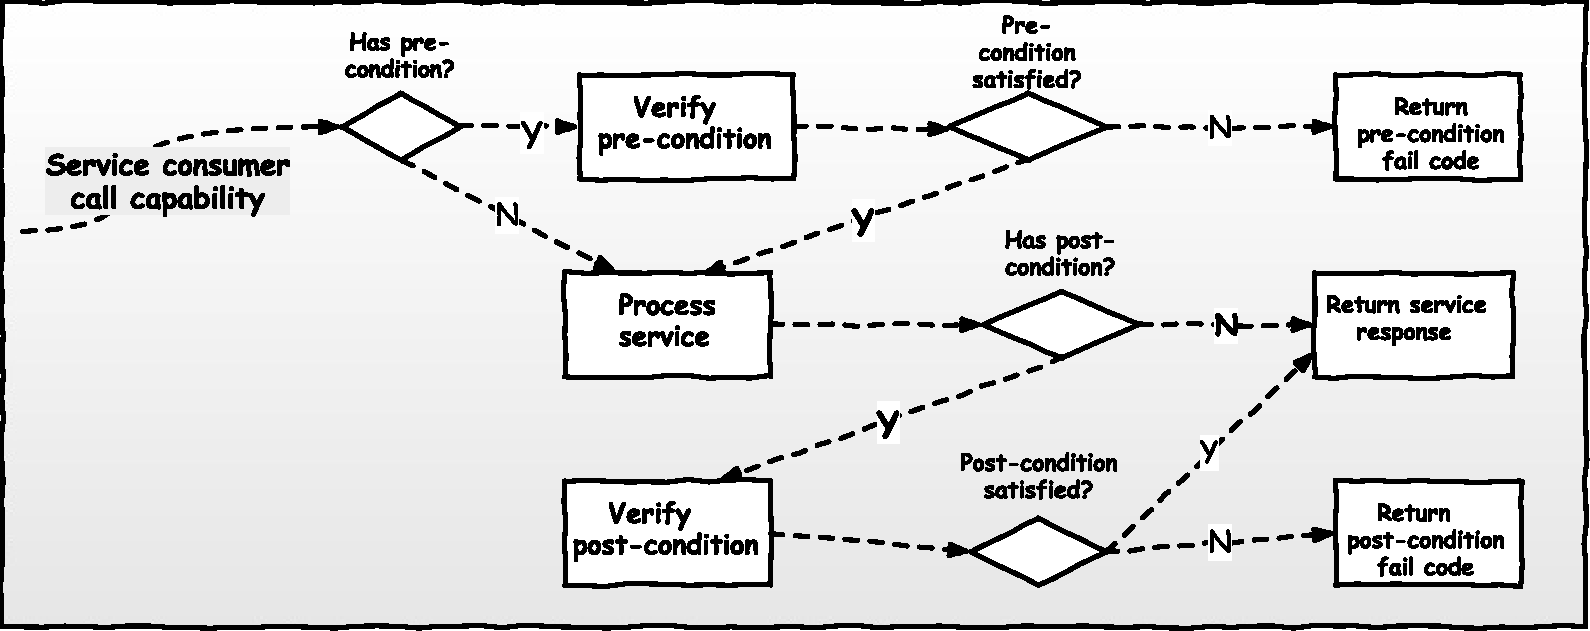
\includegraphics[width=85mm,trim = 0mm 0mm 0mm
0mm,clip]{img/FluxoDbcCondicoes.pdf} 
\caption{Digrama de atividades com verificação de pré e pós condições}
\label{FigServiceDbC}
\end{figure}

Caso tenham sido definidas pós-condições, essas são acionadas após o
processamento da capacidade, porém antes do retorno ao consumidor do serviço.
Assim, conforme Figura \ref{FigServiceDbC}, visando não entregar ao cliente uma
mensagem ou situação incoerente, as pós-condições são validadas. Caso todas as
pós-condições tenham sido satisfeitas, a mensagem de retorno é encaminhada ao
cliente. Caso contrário, será retornado o código de falha definido para a
pós-condição violada.

\subsubsection{Observação sobre invariantes}


Em \designbycontract{}, além dos conceitos de pré e pós-condições,
há também a ideia de invariantes\cite{meyer1997object}. Quando aplicadas a uma
classe em orientação a objetos, as invariantes estabelecem restrições sobre o
estado armazenado nos objetos instanciados dessa classe. No contexto de orientação a
serviços, tem-se por princípio a ausência de estados dos serviços. Por essa razão, 
no estudo sobre a incorporação de
\designbycontract{} em contratos de serviços, as invariantes não foram
consideradas.


\subsection{Verificação das precondições}


As precondições podem ser do tipo baseado nos parâmetros da requisição ou do
tipo baseado na chamada a outro serviço. Denomina-se, no contexto deste artigo,
de básica a precondição baseada apenas nos parâmetros da requisição. Essa validação é direta,
comparando os valores passados com os valores admitidos. 

No caso das precondições baseadas em serviços, é realizada chamada a outro
serviço para verificar se uma determinada condição é satisfeita. Este modo de
funcionamento, que se assemelha a uma composição de serviço, é mais versátil, pois permite
validações de condições complexas sem que a lógica associada seja conhecida pelo
cliente. Assim, os contratos que estabelecem esse tipo de
precondição se mantém simples.

A Figura \ref{FigServicePrecondition} apresenta as etapas de verificação de cada
precondição. Nota-se que a saída para as situações de desatendimento às
precondições, independentemente do tipo, é o mesma. Essa abordagem
simplifica o tratamento de exceção no consumidor.

\begin{figure}[!htb]
\centering
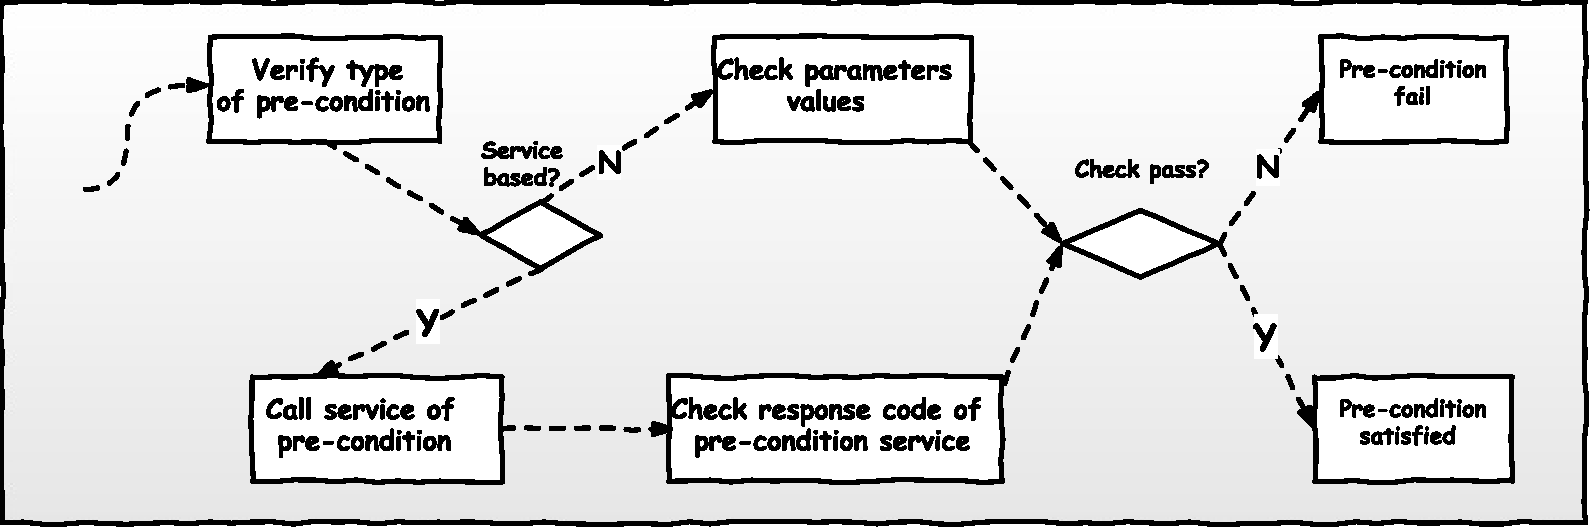
\includegraphics[width=85mm,trim = 0mm 0mm 0mm
0mm,clip]{img/FluxoPrecondicoes.pdf}
\caption{Diagrama de atividades do processamento da precondição}
\label{FigServicePrecondition}
\end{figure}


\subsection{Verificação das pós-condições}


\begin{figure}[!htb]
\centering
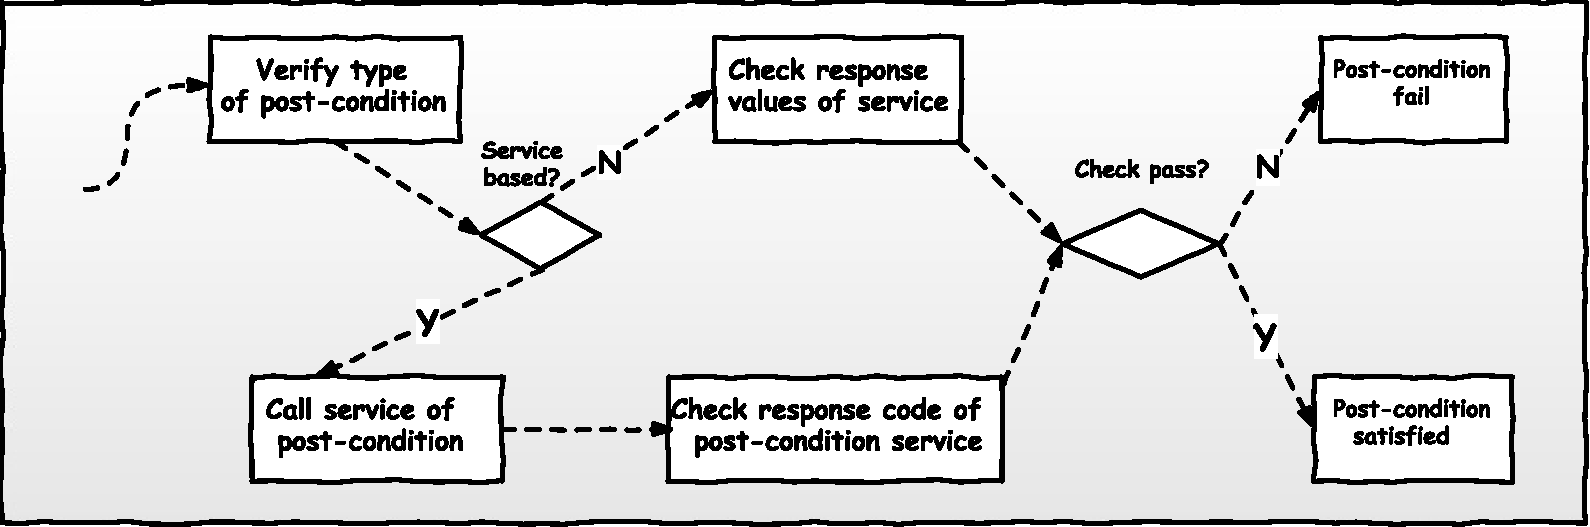
\includegraphics[width=85mm,trim = 0mm 0mm 0mm
0mm,clip]{img/FluxoPostcondicoes.pdf}

\caption{Diagrama de atividades do processamento da pós-condição}
\label{FigServicePostcondition}
\end{figure}

A verificação das pós-condições acontece de modo muito similar a das
precondições. Há também os dois tipos, baseada em valores e em chamadas a
outros serviços. O diferencial está em que a validação dos valores passa a
ocorrer a partir dos valores contidos na mensagem de retorno. A Figura
\ref{FigServicePostcondition} descreve as etapas necessárias para validação de
cada precondição.


% \subsection{Precondição básica}
% \label{precondicaoBasica}
% 
% Uma precondição básica é a que valida os valores recebidos na
% requisição, comparando-os com os valores estabelecidos na instrução
% \emph{require} do contrato. Esse tipo de precondição assemelha-se a validação
% dos atributos recebidos por um método no paradigma de orientação a objetos.
% 
% A origem das informações, isto é, onde os valores que serão validados se
% encontram, depende da operação HTTP utilizada. A Subseção \ref{FonteDadosDbc} descreve como esses
% dados são obtidos. Para realizar a comparação do valor recebido com o valor
% esperado, a \neoidl{} admite seis operadores de comparação (Subseção
% \ref{TiposContrDbC}).
% 
% \subsection{Pós-condição básica}
% 
% Em termos sintáticos, as pós-condições básicas possuem uma forma muito
% semelhante às precondições básicas (\ref{precondicaoBasica}), diferindo-se
% exclusivamente pelo uso da instrução \emph{ensure}. A Figura
% \ref{lst:DBCPosCondBasica} (linhas 8 e 9) mostra um exemplo de pós-condição
% básica em que, após a execução da operação \method{GET}, se o valor do atributo
% \emph{quantity} não for maior que zero, então o serviço não foi executado adequadamente e a exceção
% (\emph{otherwise}) é retornada.
% 
% \subsection{Precondição com chamada a serviço}
% 
% As precondições baseadas em serviços seguem uma sequência que envolve a chamada
% a outro serviço antes do processamento do serviço principal, em um tipo simples de
% composição de serviço. Essa abordagem permite que precondições complexas sejam
% validadas por serviços especializados, sem que a especificação do contrato
% de serviço se torne complexa. Essa proposta preserva ainda a ideia original de
% Eiffel\cite{meyer1988eiffel}, de que pré e pós-condições sejam expressões
% \emph{booleanas}.
% 
% A primeira etapa do processo de execução da precondição de serviço consiste em
% fazer a chamada a um serviço (ver Figura \ref{FigServicePrecondition}) por meio de uma
% operação \method{GET}. Em seguida, o código de \textit{status} retornado pelo
% serviço da precondição é comparado com o valor especificado na precondição do contrato.
% 
% Após o acionamento do serviço da precondição, o comportamento é o mesmo da
% precondição básica (ver \ref{precondicaoBasica}). Caso a precondição seja
% satisfeita, é retornado o valor indicado pela instrução \emph{otherwise}. As
% precondições de serviço na \neoidl{} admitem os mesmos operadores de comparação
% que as precondições básicas.
% 
% \subsection{Pós-condição com chamada a serviço}
% \label{Pos-condicao servico}
% 
% A pós-condição com chamada a serviço seguem a sequência de eventos indicada na
% Figura \ref{FigServicePostcondition}. No caso da pós-condição, a execução do
% serviço principal já ocorreu e a função do serviço na pós-condição é validar se
% a execução do serviço principal ocorreu com sucesso. Algumas pós-condições são
% naturais, como as que verificam se um objeto foi inserido após a operação de
% inclusão (método \method{POST}). Ou ainda, a que verifica se o objeto foi excluído
% após uma operação \method{DELETE}.

\subsection{Inclusão de condições de DbC na especificação \neoidl{}}
\label{SintaxeGeralDbc}

Um módulo \neoidl{} possui uma seção para declaração dos serviços. Cada serviço 
declarado na \neoidl{} pode ter uma ou mais
capacidades, as quais correspondem às operações HTTP utilizadas na arquitetura
REST. Sintaticamente, um serviço possui uma lista de capacidades\footnote{Os
símbolos ``['' e ``]'' identificam uma lista.}:

\begin{center}
\begin{footnotesize}
\hilight{\{\texttt{Serviço [Capacidade]}\}}
\end{footnotesize}
\end{center}

A sintaxe da \neoidl{} foi extendida para admitir a vinculação de pré e
pós-condições às capacidades. Essas contruções de \designbycontract{} são
opcionais, ou seja, uma capacidade pode não ter nenhuma pré ou pós-condição. Por
outro lado, pode-se incluir nas capacidades mais de uma precondição e mais de
uma pós-condição, simultâneamente.

\begin{center}
\begin{footnotesize}
\hilight{\{\texttt{Capacidade \textcolor{red}{[Condição DbC]}}\}}
\end{footnotesize}
\end{center}

É possível ainda, caso uma precondição ou pós-condição se aplique a todas as
capacidades de um serviço, declará-la para o serviço como um todo,
logo antes da declaração das capacidades:

\begin{center}
\begin{footnotesize}
\hilight{\{\texttt{Serviço \textcolor{red}{[Condição DbC]} [Capacidade]}\}}
\end{footnotesize}
\end{center}

 Assim, generalizando, a \neoidl{} passou a suportar a seguinte sintaxe:
 
\begin{center}
\begin{footnotesize}
\hilight{\{\texttt{Serviço \textcolor{red}{[Condição DbC]} [Capacidade
\textcolor{red}{[Condição DbC]} ]}\}}
\end{footnotesize}
\end{center}
 

\subsection{Sintaxe geral de pré e pós-condições}
\label{TiposContrDbC}

As construções de \designbycontract{} possuem as
seguintes estruturas:

\begin{center}
\begin{footnotesize}
\textbf{Condição básica:}
\hilight{\textbf{TipoCondição} \{\texttt{[Argumento
Comparação Valor]}\}}\\
\vspace{3mm}
\textbf{Condição serviço:}
\hilight{\textbf{TipoCondição} \{\texttt{Serviço (Parâmetro)
Comparação ValorSrv}\}}\\
\vspace{3mm}
\textbf{Exceção:}\\
\hilight{\textbf{Otherwise} \{\texttt{Valor de Retorno	}\}}
\end{footnotesize}
\end{center}

Onde:

\begin{itemize}
\item \textbf{TipoCondição} indica se é uma precondição (\emph{require}) ou uma
pós-condição (\emph{ensure});

\item \textbf{Argumento} indica o nome do atributo que será testado; 

\item \textbf{Comparação} indica a operação de comparação que será utilizada. A
\neoidl{}  admite seis operadores de comparação: igualdade (\literal{==}), 
diferença (\literal{<>}), maior (\literal{>}), maior ou igual
(\literal{>=}), menor (\literal{<}) e menor ou igual (\literal{<=}). Eles podem ser aplicados  a
qualquer tipo de pré ou pós-condição.

Mais de um atributo pode ser testado em uma pré ou pós-condição. Na expressão
acima, essa característica é simbolizada com a indicação de uma lista.

\item \textbf{Valor} corresponde ao valor que será comparado com o
``Argumento''.
As pré e pós-condições básicas admitem algumas combinações com os operadores
\emph{not}, \emph{and} e \emph{or}, formando expressões booleanas e,
assim, permitindo estabelecer regras mais abrangentes.

Por exemplo, a precondição apresentada na Figura \ref{lst:ModuloNeoVariosDbC} poderia
ser escrita como \emph{\textbf{require} (\textbf{not} id \literal{<=} 0)}. Os
operadores \emph{and} e \emph{or} são infixos (ex.: \emph{\textbf{require}
((id \literal{>} 0 \textbf{or} id \literal{<=} -1000))}). O uso do operador
\emph{and} produz o mesmo efeito de se declarar duas precondições.

\item \textbf{Serviço} indica o nome do serviço que será acionado. As
informações para indicação concreta da localização do serviço, ou seja, a URL de acionamento, não
são indicados nesse atributo de pre e pós-condição. Essas informações dependem
do local de implantação do serviço e não convém que estejam declaradas no
contrato, sob pena de que mudanças no ambiente de implantação do serviço gerem
impacto ao contrato.
Entretanto, caso se queira fazer essa vinculação, pode ser criada uma anotação
\neoidl{}, com essa finalidade, para o serviço.

\item \textbf{Parâmetro} tem a função de indicar os valores que serão passados
para a chamada ao serviço da pré ou pós-condição.

 \item \textbf{ValorSrv} corresponde a um valor que será comparado com o
 \textit{Status Code HTTP} retornado pelo serviço. Na \neoidl{}, esses valores
 são convencionados como o nome do correspondente ao código HTTP, com palavras
 justapostas (Ex.: ``NotFound'' tem o valor do código 404, de HTTP \textit{Not
 Found})

\item \textbf{Valor de Retorno} é utilizado na cláusula \emph{otherwise} para
indicar o valor que o serviço principal deve retornar caso uma precondiçaõ ou pós-condição
não seja atendida.

\end{itemize}

A sintaxe escolhida para possibilitar a especificação de pré e pós condições
na \neoidl{} foi influenciada por três linguagens e extensões de linguagens de
programação: Eiffel, JML e Spec\# 


\subsection{Um exemplo de módulo com \designbycontract{}}

A Figura \ref{lst:ModuloNeoVariosDbC} apresenta um exemplo de módulo \neoidl{}
de um serviço completo com três operações, cada uma com duas
condições de \designbycontract{}.

A operação \method{GET} possui uma precondição em que o valor do atributo \emph{id} 
deve ser maior que zero (linha 8), caso contrário a operação deve retornar o valor
correspondente a ``NotFound''. Uma pós-condição assegura que, se o serviço for
executado adequadamente, o valor de \emph{quantity} será maior que zero (linha
9). Se for violada a pós-condição, a operação \method{GET} retorna o valor
``NoContent''.

A operação \method{POST} possui duas precondições (linhas 13 e 14). A primeira,
básica, valida o valor do atributo \emph{quantity}. A segunda, aciona o serviço
\emph{store.getOrder} com o parâmetro \emph{id}. Nessa operação, foi
definido um valor de exceção único para as duas precondições. A \neoidl{}
associa essa instrução de \emph{otherwise} geral às instruções anteriores que
não possuem condição e exceção específica (caso da linha 8).

Na operação \method{DELETE} foi utilizado o operador lógico \emph{and} na
precondição (linha 18). A pós-condição faz a chamada ao serviço
\emph{store.getOrder}. Tanto a pré como a pós-condição possuem o mesmo valor de
exceção (linha 20). 

\begin{figure}[htb]
\begin{scriptsize}
\lstinputlisting[language=NeoIDL,firstnumber=1]{trechos_codigo/store_dbc_complete.neo}
\end{scriptsize}
\caption{Exemplo de módulo \neoidl{} com várias instruções de \designbycontract{}}
\label{lst:ModuloNeoVariosDbC}
\end{figure} 	



\subsection{Fontes de dados para pré e pós-condições}
\label{FonteDadosDbc}

Os serviços REST na \neoidl{} seguem uma convenção em relação ao conteúdo
presente na requisição e na resposta para cada tipo de operação \emph{HTTP}.
Por exemplo, o método \method{GET}
submete os argumentos pelo \emph{path} ou como \textit{query string} da
requisição e não em seu corpo. A Figura \ref{Fig:FonteDadosDbcNeoIDL} resume a origem para cada operação.

Há diferenças também entre os tipos básico e baseado em serviços das construções
de \designbycontract{}. As operações \method{GET} e \method{DELETE} não possuem
argumentos encaminhados no corpo da requisição, de modo que os argumentos são
retirados do \emph{path} ou \emph{query string} para va\-li\-da\-ção das precondições, 
tanto no tipo básico como no tipo baseado em
composição. Na figura, essa origem é identificada como \textit{Request arguments}.

\begin{figure}[!htb]
\centering
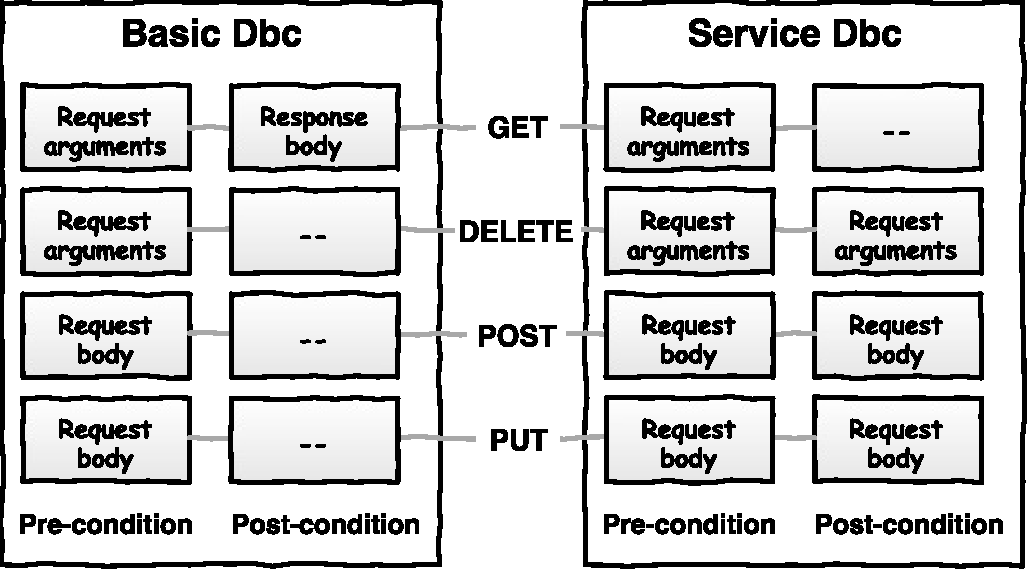
\includegraphics[width=65mm,trim = 0mm 0mm 0mm
0mm,clip]{img/FonteDadosDbcNeoIDLIngles.pdf}
\caption{Diagrama da fonte de dados para acionamento de pré e pós-condições}
\label{Fig:FonteDadosDbcNeoIDL}
\end{figure}


Por outro lado, as operações \method{POST} e \method{PUT} submetem os dados a
serem inseridos ou alterados pelo corpo da requisição (\textit{Request body}),
local de onde as precondições básicas e baseadas em serviços devem extrair os
parâmetros de validação.
A \neoidl{} utiliza a notação JSON\cite{JSon} no corpo das requisições. A
representação dos argumentos utiliza o padrão separado por pontos para indicar
elementos mais internos (ex. ``Pessoa.Nome'').

No caso das pós-condições, a origem das informações diverge entre o tipo
básicos e o tipo por serviços. A única operação que admite pós-condição básica é
a operação \method{GET}, em que os argumentos de validação são extraídos do
corpo da resposta (\textit{Response body}). As demais operações não retornam dados
no corpo da requisição, pois estão voltadas para alteração e não consulta de
informações. Além disso, não há utilidade em se validar dados de requisição
em uma pós-condição.

Já as pós-condições baseadas em serviços não suportam a operação \method{GET}.
Embora seja tecnicamente possível acionar um serviço com base nos argumentos da
requisição, como não se tem modificação nos dados por essa operação, a
validação dessas informações pode se dar por meio de serviço deve ser feita nas
precondições. Ademais, as pós-condições básicas da operação \method{GET} cumprem
com o objetivo que validar as informações de saída.

A pós-condição da operação \method{DELETE} pode acionar serviços com base nos
argumentos da requisição (\textit{Request arguments}). Um caso típico é de
acionar o serviço de consulta para verificar se o dado foi efetivamente
excluído. As operações \method{POST} e \method{PUT} podem acionam serviços em
pós-condições utilizando as informações do corpo da requisição (\textit{Request
body}), uma vez que essas operações não possuem dados no corpo da resposta. 
 
\subsection{Estudo de caso: plugin Twisted}
\label{pluginTwisted}

A incorporação de regras de \designbycontract{} aos contratos para
serviços REST escritos em \neoidl{} elevam a um novo patamar os níveis de
garantias com a estabilidade comportamental dos serviços. Nesse sentido, a
preocupação em garantir ao cliente que o serviço proverá as informações de que
ele necessita aumenta, reforçando os benefícios observados com a prática
\CtFirst{}. Ou seja, o desenho do serviço considera ainda mais a perspectiva do
consumidor do serviço.

O contrato, porém, é apenas uma especificação, no
sentido de descrever regras e não de torná-las executáveis em si. Todavia, a
\neoidl{} é, além de uma linguagem formal, um \framework{} de geração de
código poliglota por meio de \textit{plugins}.

Para se comprovar a viabilidade de se conceber serviços com suporte a pré e
pós-condições, foi desenvolvido, no decorrer da pesquisa de mestrado, um
\textit{plugin} da \neoidl{} que cumpre com tal finalidade. As próximas
subseções detalham como é estruturada a arquitetura do serviço gerado e seu comportamento em relação a
\designbycontract{}. Ao final, alguns aspectos sobre a implementação do
próprio \textit{plugin} são descritos.

Adotou-se o \framework{} \emph{Python Twisted}\cite{fettig2005twisted} como tecnologia para
construção dos serviços com pré e pós-condições. A escolha se deu em razão de
\twisted{} possuir uma arquitetura voltada para processamento de requisições de vários
tipos de protocolos de rede sobre uma infraestrutura simples e autônoma. 

\subsection{Arquitetura dos serviços \twisted{}}
\label{ArquiteturaTwisted}

Os serviços \twisted{} gerados pela \neoidl{} são estruturados em uma
arquitetura que extende a arquitetura base do \twisted{} \emph{Reactor},
incorporando serviços ao processamento das requisições. Os serviços são autônomos entre si, e
processam as requisições de acordo com o roteamento realizado pelo servidor.

Em termos de classes, a \neoidl{} gera um conjunto de três módulos base,
que constituem o pacote do \twisted{} \textit{server}, representados na
parte superior da Figura \ref{Fig:TwistedArchtecture}. Essas classes são fixas,
ou seja, não dependem da quantidade nem do conteúdo dos serviços declarados no
módulo \neoidl{}.

A classe \emph{Server} é o núcleo do \twisted{} \textit{server}. Ela é
responsável por fazer executar o servidor HTTP, receber as requisições,
identificar as operações da requisição (\method{GET}, \method{POST}, \method{PUT} ou \method{DELETE}), e
direcionar a requisição para o serviço específico. A identificação do serviço é
feita por meio de um arquivo de rota (routes.json), o qual possui uma tradução
entre os \emph{paths} das requisições e os serviços responsáveis por cada uma
delas.

A classe \emph{Utils} contém um conjunto de funções utilitárias, como a que
realiza o \textit{parse} da requisição para extrair os argumentos repassados
na URI ou \textit{query string}. Ela também define o objeto que trafega a
resposta dos serviços entre os serviço e o servidor.

Essas duas classes são suficientes para o servidor quando não se utiliza
\designbycontract{} nos serviços. O pacote
\emph{DbcConditions} consolida o conjunto de classes res\-pon\-sá\-veis por
processar as pré e pós-condições. A principal função de \emph{DbcConditions} é realizar a
comparação entre o valor real e o valor esperado, efetivando toda a
lógica corresponde às construções de \designbycontract{} descritas na Subseção
\ref{TiposContrDbC}.

\begin{figure}[htb]
\centering
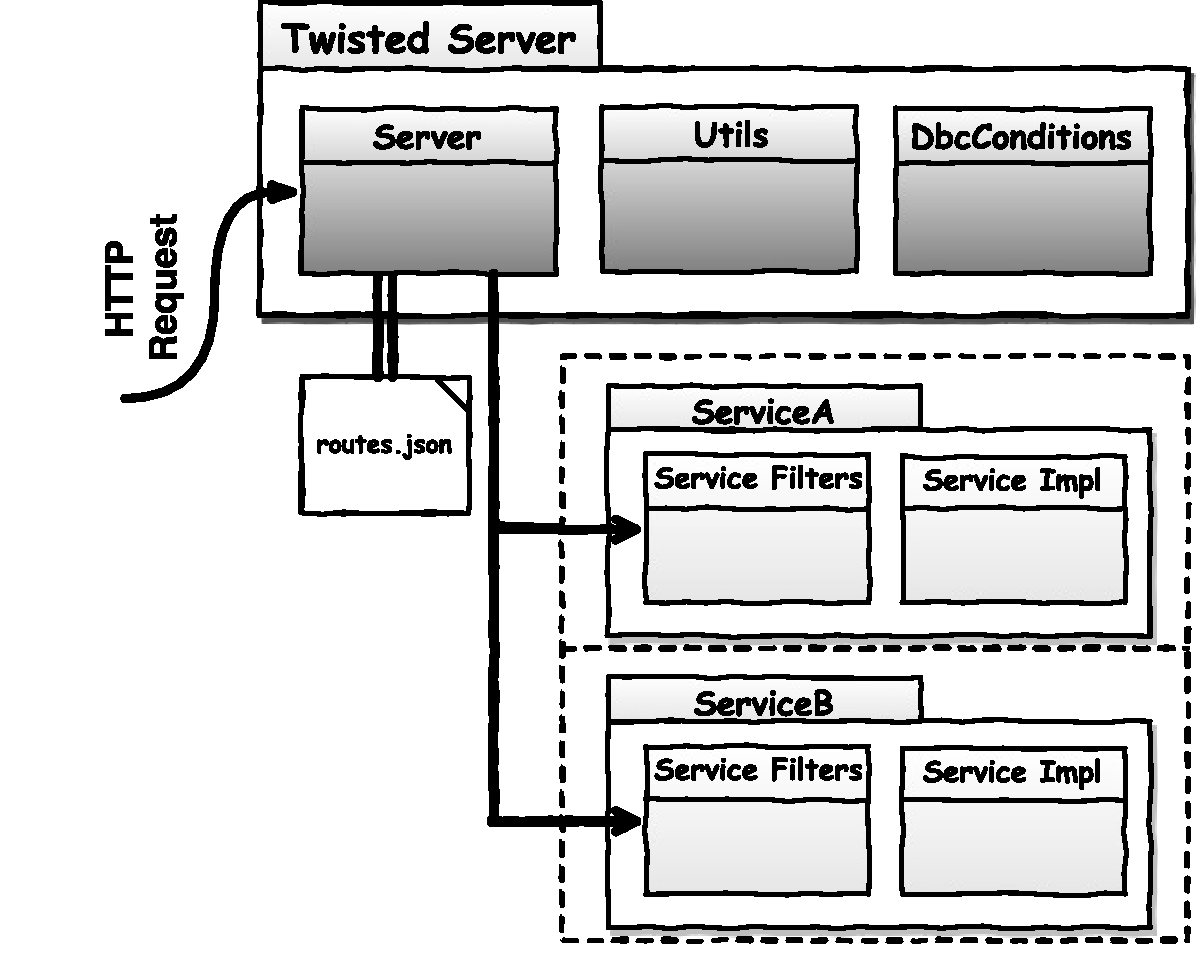
\includegraphics[width=70mm,trim = 18mm 4mm 0mm
0mm,clip]{img/TwistedServer.pdf}
\caption{Arquitetura do serviço Twisted gerado pela \neoidl{}}
\label{Fig:TwistedArchtecture}
\end{figure}

Em \emph{DbcConditions} estão as funções que carregam a lista de pré e
pós-condições para cada serviço. A chamada para as pré e pós-condições baseadas
em serviços também é construída nesse pacote. Esse pacote é fundamental para o
funcionamento das cons\-tru\-ções de \designbycontract{}.

Para cada serviço declarado no módulo \neoidl{} são geradas duas classes: os
filtros do serviço e o serviço em si. A classe \emph{ServiceFilter} recebe a
requisição; carrega e processa as precondições; aciona o serviço e; ao final,
carrega e processa as pós-condições. Esse modo de operação dos filtros é
ilustrado na Figura \ref{Fig:TwistedFiltes}. A classe do serviço, por
fim, contém apenas a estrutura para implementação da lógica interna do serviço.

\begin{figure}[!htb]
\centering
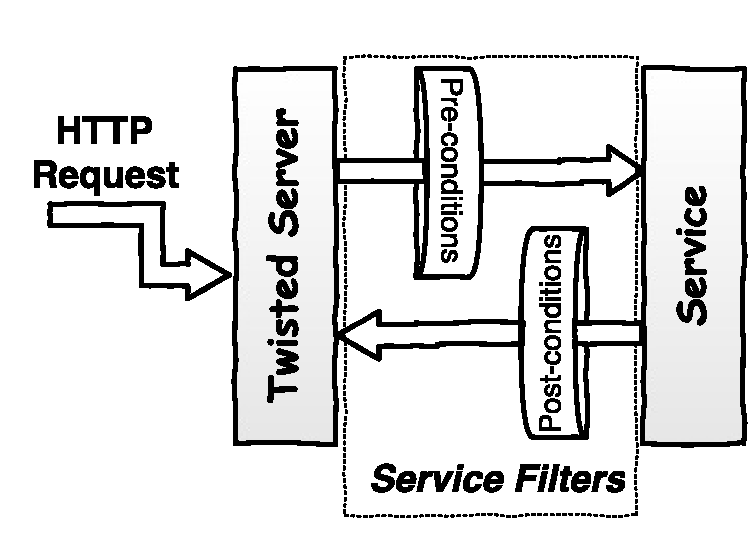
\includegraphics[width=45mm,trim = 5mm 6mm 0mm 
3mm,clip]{img/TwistedFilters.pdf}
\caption{Modo de operação das pré e pós-condições no serviço Twisted}
\label{Fig:TwistedFiltes}
\end{figure}

\subsection{Geração de código}

O plugin \twisted{} é um conjunto de seis módulos Haskell. Para cada tipo de
arquivo gerado, há um módulo no \textit{plugin}, conforme Figura
\ref{PluginTwisted}.
Os módulos \emph{PPService}, \emph{PPUtils} e P\emph{PDbcConditions} apenas
imprimem um código Python fixo, sem qualquer interferência do módulo \neoidl{}
processado. \emph{PPRoute} é um pequeno módulo (42 linhas) que processa as
informações contidas nas instruções \emph{path} dos serviços declarados no
módulo \neoidl{} e mapeia a correspondência entre as URIs e os serviços.

\begin{figure}[!htb]
\centering
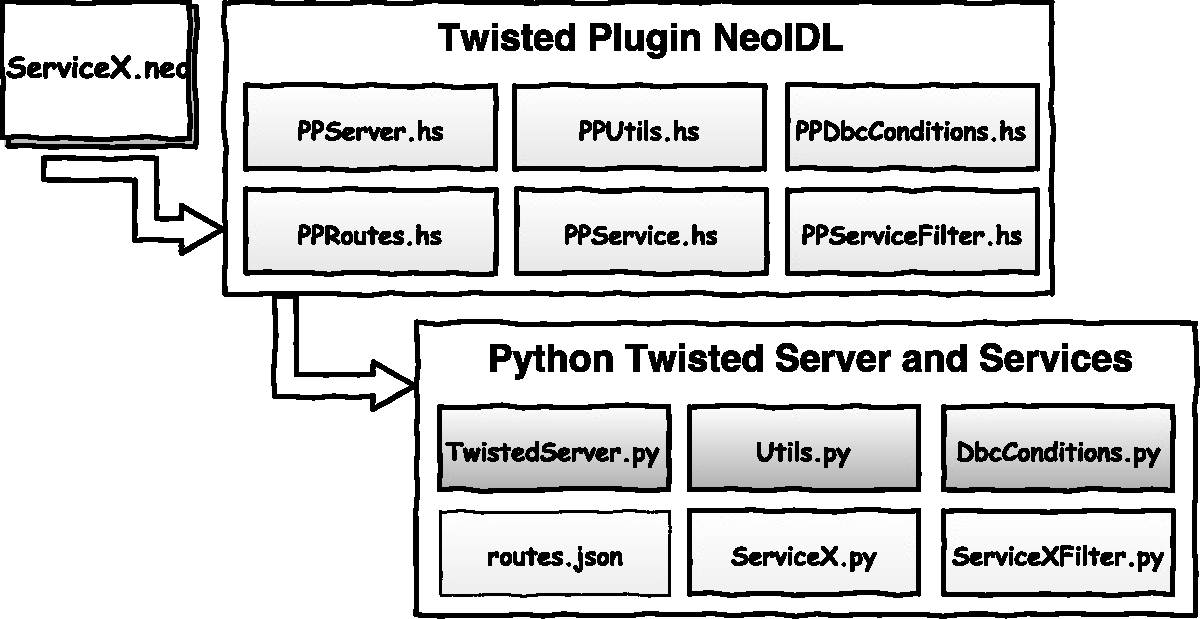
\includegraphics[width=85mm,trim = 0mm 0mm 0mm 
0mm,clip]{img/PluginTwisted.pdf}
\caption{Plugin para geração de código Twisted com suporte a \designbycontract{}}
\label{PluginTwisted}
\end{figure}

O módulo \emph{PPService} gera uma classe com um método para cada operação do
serviço. Na versão atual do \textit{plugin}, os métodos são implementados com
uma lógica de gravação de objetos em um banco em memória, apenas para simplificar o teste
dos código gerado. Essa implementação não é relevante, uma vez que a lógica
especializada do serviço real a substituirá.

A parte correspondente ao acionamento das pré e pós-condições é produzido pelo
módulo \emph{PPServiceFilter}. O código produzido por este módulo é composto de
duas seções: (i) a declaração das condições de \designbycontract{} e (ii) o
carregamento dessas condições. A primeira seção, de declaração das condições
\designbycontract{} contém a lista de pré e pós-condições do serviço. A Figura 
\ref{Fig:LhsRhsDbcConditions} apresenta um exemplo de condição especificada em
\neoidl{} transformada em código \emph{Python Twisted}.

O lado esquerda dessa
figura contém a especificação de uma pós-condição (\emph{\textbf{ensure}}, na
linha 2) associada à operação \method{GET} (linha 1). Constitui-se de uma
pós-condição básica, que testa se o valor de resposta \emph{quantity} é maior que zero
(linhas 3 a 5). Caso a pós-condição não seja satisfeita, o serviço retorna o
código \emph{HTTP No Content}.


\setbox0=\hbox{%
%\begin{minipage}{1.9in}
\begin{minipage}{3.5cm}
\begin{lstlisting}[
basicstyle={\tiny\ttfamily},
identifierstyle={\color{black}},
tabsize=2,
language={NeoIDL},
numbersep=8pt,
numbers=left,
xleftmargin=0.5cm,frame=tlbr,framesep=2pt,framerule=0pt,
morekeywords ={class,run}
]
@get Order getOrder (int id)
		ensure (
				quantity
				>
				"0"
		),
		otherwise "NoContent";
\end{lstlisting}
\end{minipage}
}
\savestack{\listingA}{\box0}

\setbox0=\hbox{%
\begin{minipage}{4.2cm}
\begin{lstlisting}[
basicstyle={\tiny\ttfamily},
identifierstyle={\color{black}},
tabsize=2,
language={PythonTwisted},
numbersep=8pt,
numbers=left,
xleftmargin=0.5cm,frame=tlbr,framesep=2pt,framerule=0pt,
morekeywords ={class,run}
]
self.list.append(
	DbcCheckBasic(
		'quantity',
		'>',
		'0',
		204,
		ValuesSource.responseBody,
		DbcConditionType.PostCondition,
		OperationType.GET
	)
)
\end{lstlisting}
\end{minipage}
}
\savestack{\listingB}{\box0}

\begin{figure}[h]
\begin{center}
\begin{tabular}{|c|c|}
\hline
%\stackinset{l}{-5pt}{t}{13\llength}{$\bullet$}{\listingA} &
%\stackinset{l}{-5pt}{t}{ 7\llength}{$\bullet$}{\listingB} \\
\stackinset{l}{-5pt}{t}{}{}{\listingA} &
\stackinset{l}{-5pt}{t}{}{}{\listingB} \\
\hline
\end{tabular}

\caption{Transformação de pós-condição \neoidl{} (lado esquerdo) em código
Python \twisted{} (lado direito)}
\label{Fig:LhsRhsDbcConditions}
\end{center}
\end{figure}

Do lado direito da Figura \ref{Fig:LhsRhsDbcConditions} está o código
\emph{Python Twisted} correspondente. O motor de transformação identifica que a
condição especificada é uma pós-condição básica (classe \emph{DbcCheckBasic} na linha 2
e tipo na linha 8) associada uma operação \method{GET} (linha 9). Conforme
convenção adotada sobre a fonte de informações (Subseção \ref{FonteDadosDbc}), a
pós-condição é carregada com a indicação de que os argumentos devem ser lidos do
corpo da resposta do serviço (linha 7).

% Os parâmetros da pós-condição possuem uma correspondência direta, em que as
% linhas 3 a 5 do lado esquerdo correspondem também às linhas 3 a 5 do lado
% direito. O valor de exceção da especificação \neoidl{} é traduzido no código
% HTTP correspondente (linha 6). Ambos os códigos apresentados na Figura
% \ref{Fig:LhsRhsDbcConditions} são, na realidade, escritos em uma única linha.
% O uso de múltiplas linhas foi adotado aqui apenas para efeitos didáticos.

A segunda seção da classe \emph{ServiceFilter} é genérica para
qualquer serviço. A Figura \ref{lst:filtrosServicosTwisted} contém um trecho
dessa seção. Cada método se inicia com o carregamento das precondições (linha
10), seguindo pelo acionamento do serviço principal (linha 12). Por fim,
as pós-condições são carregadas (linha 14).

\subsection{ESTUDO EMPÍRICO SUBJETIVO} 
\label{analiseSubjetiva}

% Há diversas formas e técnicas para se conduzir um estudo empírico, cada uma com
% suas vantagens e desvantagens \cite{shull2008guide}. Nas técnicas diretas, o pesquisador
% atua de forma explícita e perceptível pela equipe do projeto de \textit{software}, interagindo
% com eles em maior ou menos grau. As técnicas indiretas são caracterizadas pelo
% acesso indireto do pesquisador aos participantes, por meio da captura de
% informações do ambiente de trabalho deles. Há ainda a abordagem independente,
% em que se analisa apenas o produtos de trabalho, como documentação e código
% fonte.
% 
% As técnicas diretas são divididas em inquisitivas e de observação.
% \textit{Brainstorming}, grupo focais, entrevistas, questionários e modelagem
% conceitual estão entre as técnicas inquisitivas. Essas são, muitas vezes, a
% única forma de obter o engajamento dos envolvidos na realização das atividades.
% Entretanto, elas tem o risco de serem excessivamente subjetivas e de medição de
% resultados pouco precisa.
% 
% A abordagem observatória está ligada a técnicas como seções de
% \textit{think-aloud}\footnote{Momentos em que os participantes são
% convidados a expressar seus pensamentos em voz alta (`pensar alto'), a partir de
% questões levantadas pelo investigador}, sombreamento\footnote{Consiste
% em acompanhar o participante na realização de todas as suas atividades} e
% participante-observador (em que o pesquisar participa realizando 
% atividades chave para o projeto).
% As técnicas observatórias permitem um estudo em tempo real dos fenômenos. Porém, elas levam a uma fase de análise
% difícil, pois geram muitas informações e requerem um elevado conhecimento para
% se interpretar corretamente os dados.

A meta de investigar a utilidade do uso de construções de \designbycontract{} na
\neoidl{} estruturada conforme o método GQM é apresentada na Tabela
\ref{TabelaMetasGQM}.

\begin{table}[h]
\centering
\begin{tabular}{r|lr}
\multicolumn{2}{c}{GQM}\\
\hline    
Analisar & contratos especificados em NeoIDL \\
Com o propósito de  & avaliá-los \\
Com relação a & facilidade de uso e utilidade das construções \\
& de \designbycontract{} \\
Do ponto de vista de & arquitetos e desenvolvedores experientes \\
No contexto de & um serviço real.           
\end{tabular}
\caption{Meta de investigar o uso de Dbc na \neoidl{} estruturado conforme
método GQM}
\label{TabelaMetasGQM}
\end{table}

O modelo escolhido para subsidiar a elaboração das perguntas foi o
\textit{Technology Acceptance Model} -- TAM, proposto por Davis em 1989
\cite{davis1989perceived} e que possui uma sólida base teórica e ampla
utilização.
O principal objetivo do modelo TAM é identificar os motivos que levam à aceitação
ou rejeição de uma tecnologia. O modelo está estruturado em dois conceitos:
percepção da utilidade (\textit{perceived usefullness} - PU) e percepção sobre a
facilidade de uso (\textit{perceived ease of use} - PEU)
\cite{hernandes2010avaliaccao}.

Percepção de utilidade é medido com o grau em que uma pessoa acredita que
utilizar uma determinada tecnologia vai melhorar sua eficiência em suas
atividades. A percepção de facilidade está relacionada ao grau em que uma pessoa
acredita que determinada tecnologia será livre de esforço. Adicionamente, alguns
estudos incluem um outro aspecto, que é a predisposição ao uso
(\textit{self-predicted future usage}), que está relacionado à indicação da 
preferência de uma determinada tecnologia em detrimento de outras \cite{laitenberger1998evaluating}.

As respostas normalmente são
escalas que vão desde a discordância total até a concordância total quanto a
afirmação apresentada. Essa escala é denominada \textit{Likert Scale}
\cite{allen2007likert}. As respostas são agrupadas para se avaliar se, no
conjunto, as respostas mais favoráveis indicam uma tendência de aceitação. O
processo de elaboração do questionário é apresentado na Subseção \ref{ModelagemQuestionario}.

A distribuição do questionário foi feita por formulário eletrônico publicado na
Internet, utilizando a ferramenta \textit{Google Forms}. Essa ferramenta
simplifica o processo de escrita do questionário e também a consolidação das
informações. O \textit{link} para acesso ao questionário foi encaminhado a
grupos de arquitetos e desenvolvedores cujo nível técnico elevado era de
conhecimento dos pesquisadores. O questionário ficou disponível para respostas
por um período de três semanas, até que atingisse um volume de respostas satisfatório.

\subsection{Questionário}

O questionário foi organizado em três seções: a primeira seção têm cinco
perguntas para traçar o perfil do respondente, principalmente em relação a sua
experiência técnica; a segunda seção, com três perguntas, faz uma avaliação
sobre especificação formal de contratos e a sintaxe da
\neoidl{} e de Swagger \cite{swaggerSite}; 
Oito questões formam a última seção, a qual dá enfoque ao principal ponto, que é
a avaliação das utilidade do uso de \designbycontract{} na \neoidl{}.

Na primeira seção do questionário, a pergunta sobre o local de prestação de serviços tem a finalidade de 
identificar e, na fase de análise, eliminar respostas oriundas de locais para os quais o questionário
não foi submetido, pois este não exigia autenticação. A segunda e terceira
questões visam mapear se o respondente possui experiência e
conhecimento suficiente para responder adequadamente o questionário. A questões
quatro e cinco pretendem indicar o nível de especialização em \wss{} REST e
na linguagem Swagger.

A partir da segunda seção do questionário, o
método TAM foi utilizado para nortear a elaboração das
perguntas.
O questionário TAM foi adaptado ao cenário de avaliação da aceitação de uma DSL,
pois, durante a pesquisa, não foram identificados estudos que utilizam TAM para
fazer estudo idêntico. Entretanto, a aplicação de TAM abrange um campo vasto
e as questões pode ser adaptadas ao objeto de estudo \cite{babar2007evaluating},
desde que os aspectos base do método sejam mantidos.

A base da segunda seção do questionário é um conjunto de especificações de
serviços. Inicialmente, é apresentada em texto
descritivo, a especificação de um serviço que deve recuperar uma lista de
informações, desde que atendida uma condição. Em seguida, o mesmo serviço é especificado em Swagger. Na sequência, a
especificação é feita em \neoidl{}. Ao final, um trecho do código Java que
implementa o serviço real é apresentado.

Como a \neoidl{} é uma DSL muito pouco conhecida, foram acrescentadas questões
sobre a sua expressividade, pois essa característica é considerada o principal
critério para a escolha de uma linguagem \cite{mackinlay1985expressiveness}. O
quão fácil é idenficar os elementos da linguagem e compreender o que eles
representam é fundamental para se decidir usar uma DSL. Além disso, espera-se de uma DSL, por
não ter o compromisso de atender a propósitos gerais, que ela seja mais
acessível \cite{taha2008domain}. 

A terceira seção é a principal, pois enfoca na utilização de construções de
\designbycontract{} em contratos REST. Essa seção possui uma parte introdutória
onde é apresentada uma conceituação de \designbycontract{}. Em seguida, é
apresentada a especificação de serviço da seção anterior em \neoidl{}
acrescentando a ela	 as construções de \designbycontract{}. Após essa parte
introdutória, são feitas quatro questões (9 a 12) sobre a simplicidade e
utilidade do novo contrato em \neoidl{}.

Na sequência, é apresentado um trecho curto sobre geração automática de código a
partir de especificações formais. O propósito dessa parte é tratar também da
utilidade do recurso de geração de código provido pela \neoidl{}. Duas perguntas
são feitas sobre esse ponto (13 e 14). Por fim, são feitas duas afirmações (15
e 16) sobre a predisposição ao uso futuro da \neoidl{}.

\subsection{Análise dos Resultados}
\label{AnaliseQuestionario}


Esta subseção apresenta e discute os resultados do questionário aplicado. As
respostas são avaliadas em grupos, iniciando pela avaliação do perfil de
respondentes. Em seguida, são avaliadas as questões 6 a 8, sobre a especificação
formal de contratos e a expressividade de Swagger e \neoidl{}. As respostas às
questões 9 a 12, sobre a aplicabilidade de \designbycontract{} na especificação
 de contratos REST, são debatidos na sequência. A penúltimo grupo trata da
 geração de código com \designbycontract{}, com as questões 13 e 14. Por fim,
 são discutidas as duas últimas questões, sobre predisposição ao uso.

\subsubsection{Perfil dos respondentes}

A primeira questão tinha o objetivo de apenas identificar respostas
submetidas por pessoas fora do público alvo. Cinco instituições das quais se
conhecia o nível técnico e com as quais se tinha contato com profissionais
concentraram a maior parte das respostas. As demais respostas são empresas
relacionas a essas instituições, por indicação de técnicos experientes
do primeiro grupo. Sob este aspecto, nenhuma das respostas foi considerada
anormal e, portanto, todas foram validadas, totalizando 26 respondentes.

A segunda questão levantou o tempo de experiência dos respondentes com
desenvolvimento de sistemas Web. O resultado foi sumarizado na Tabela
\ref{quantidadeRespostas2}. Como o público alvo, definido na meta GQM (Tabela
\ref{TabelaMetasGQM}), é de desenvolvedores experientes, os respondentes que
apontaram experiência inferior a três anos estão fora do perfil esperado e suas
respostas foram descartadas (linhas em cinza). Assim, o questionário teve um
conjunto de 21 respostas válidas.

\begin{table}[!bth] 
\centering
\scriptsize
\begin{tabular}{p{3cm}|p{1cm}}
\hline   
Experiência com desenvolvimento Web& Q2 \\
\hline   
\cellcolor{light-gray}Não tenho experiência &  \cellcolor{light-gray}2  \\
\cellcolor{light-gray}Entre 1 e 2 anos      &  \cellcolor{light-gray}3  \\
Entre 3 e 4 anos      &  1  \\
Entre 5 e 6 anos      &  3  \\
Entre 7 e 8 anos      &  5  \\
Entre 9 e 10 anos     &  1  \\
Há mais de 10 anos    & 11  \\
\end{tabular}
\caption{Respostas sobre a experiência com desenvolvimento Web}
\label{quantidadeRespostas2}
\end{table}

A terceira questão identificou o conhecimento dos respondentes com
desenvolvimento de \wss{}. Conforme apresentado na Tabela
\ref{quantidadeRespostas3}, as respostas estão polarizadas, em que 40\%
(quarenta por cento) tem nenhuma ou pouca experiência (menos de dois anos). Por
outro lado, 23\% (vinte e três por cento) dos respondentes possui experiência
muito alta (mais de 10 anos). Caso o volume de respostas fosse muito grande (mais de
200 pessoas), poderia ser feita uma análise comparativa da \neoidl{} de acordo
com a experiência de \ws{}.


\begin{table}[!bth] 
\centering
\scriptsize
\begin{tabular}{p{3cm}|p{1cm}}
\hline   
Experiência com \ws{} & Q3 \\
\hline   
Não tenho experiência &  3  \\
Entre 1 e 2 anos      &  5  \\
Entre 3 e 4 anos      &  6  \\
Entre 5 e 6 anos      &  2  \\
Entre 7 e 8 anos      &  0  \\
Entre 9 e 10 anos     &  0  \\
Há mais de 10 anos    &  5  \\
\end{tabular}
\caption{Respostas sobre experiência com \wss{}}
\label{quantidadeRespostas3}
\end{table}        

A questão quatro identificou o conhecimento e experiência do respondente com o
modelo arquitetural REST. Apenas dois (menos de 10\%) respondentes não tem
experiência alguma com desenvolvimento de \wss{} REST, como pode ser verificado na Tabela
\ref{quantidadeRespostas4}. Outros 42\% (quarenta de dois por cento) dos
respondentes, porém, tem experiência e conhecimento sobre os padrões arquiteturais que formam
o modelo REST.

\begin{table}[!bth] 
\centering
\scriptsize
\begin{tabular}{p{6cm}|p{1cm}}
\hline   
Experiência com REST & Q4 \\
\hline   
Nunca desenvolvi com a tecnologia &  2  \\
\cellcolor{light-gray}Já desenvolvi serviços algumas APIs REST, mas não conheço
a especificação & \cellcolor{light-gray}7 \\
Tenho experiência superior a dois anos em desenvolvimento REST, mas não conheço
a especificação & 3 \\
\cellcolor{light-gray}Tenho experiência superior a dois anos em desenvolvimento
REST e conheço a especificação &  \cellcolor{light-gray}9  \\

\end{tabular}
\caption{Respostas sobre conhecimento e experiência com REST}
\label{quantidadeRespostas4}
\end{table}

A última questão sobre o perfil do respondente tratou do conhecimento e
experiência com a especificação de contratos em Swagger. O conjunto de respostas
confirmou a tendência pelo mercado pela uso de Swagger. Mais de 70\% (setenta
por cento) dos respondentes já tiveram algum contato com especificação de
contratos em Swagger (Tabela \ref{quantidadeRespostas5}). Esse cenário indica
que o conjunto de profissionais é qualificado e possui capacidade crítica para
responder às demais questões.

\begin{table}[!bth] 
\centering
\scriptsize
\begin{tabular}{p{6cm}|p{1cm}}
\hline   
Experiência com Swagger & Q5 \\
\hline   
Não sei do que se trata ou apenas ouvi a respeito & 6 \\
Já tive contato com especificações em Swagger & 8 \\ 
Já especifiquei APIs REST em Swagger &  5  \\
Tenho experiência superior a um ano em Swagger & 2 \\


\end{tabular}
\caption{Conhecimento e experiência dos respondentes com Swagger}
\label{quantidadeRespostas5}
\end{table}

  
   

\subsubsection{Análise da especificação de contratos formais e expressividade
de Swagger e \neoidl{}}

A partir da questão 6, as respostas foram dadas na escala \textit{Likert} sobre
as afirmações colocadas. Os dados foram processados com utilização do software
estatístico R, com o objetivo de apresentar os resultados por meio de gráficos
que facilitam a interpretação de tendência. A cor vermelha é utilizada para
indicar discordância sobre as afirmações, sendo que o vermelho mais escuro
corresponde a discordância total. Da mesma forma, a cor azul é utilizada para
indicar concordância.

Na questão 6 foi apresentada uma afirmação sobre a efetividade de se especificar
contratos formalmente, em detrimento de especificação textual descritiva.
Conforme apresentado na primeira barra da Figura \ref{Respostas6a8},
praticamente todos os respondentes concordaram com a afirmação e nenhum
discordou. Esse resultado reforça a utilidade de se utilizar contratos
formais para especificação de serviços.


\begin{figure}[!htb]
\centering
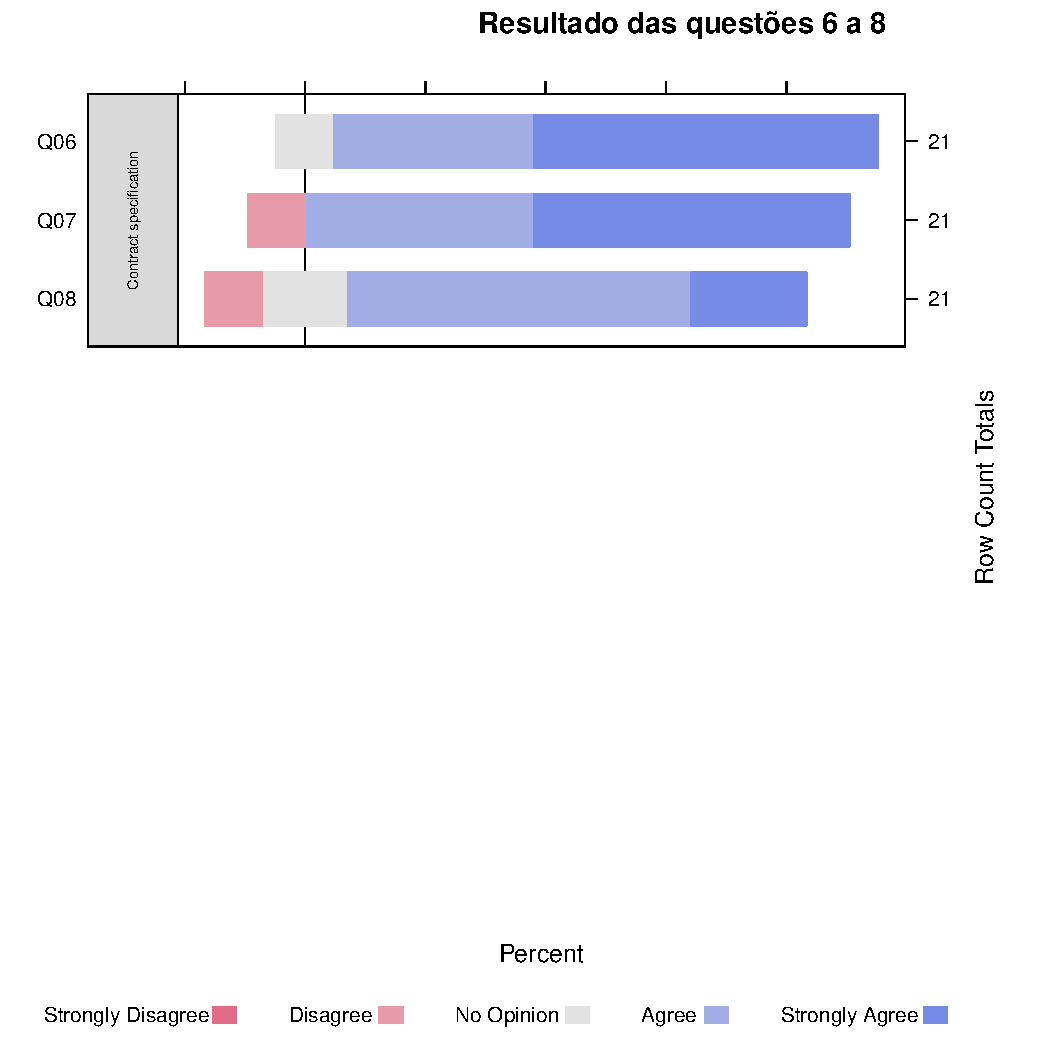
\includegraphics[width=85mm,trim = 6mm 115mm 6mm 
10mm,clip]{img/GraficoResultadoQuestoes6a8.pdf}

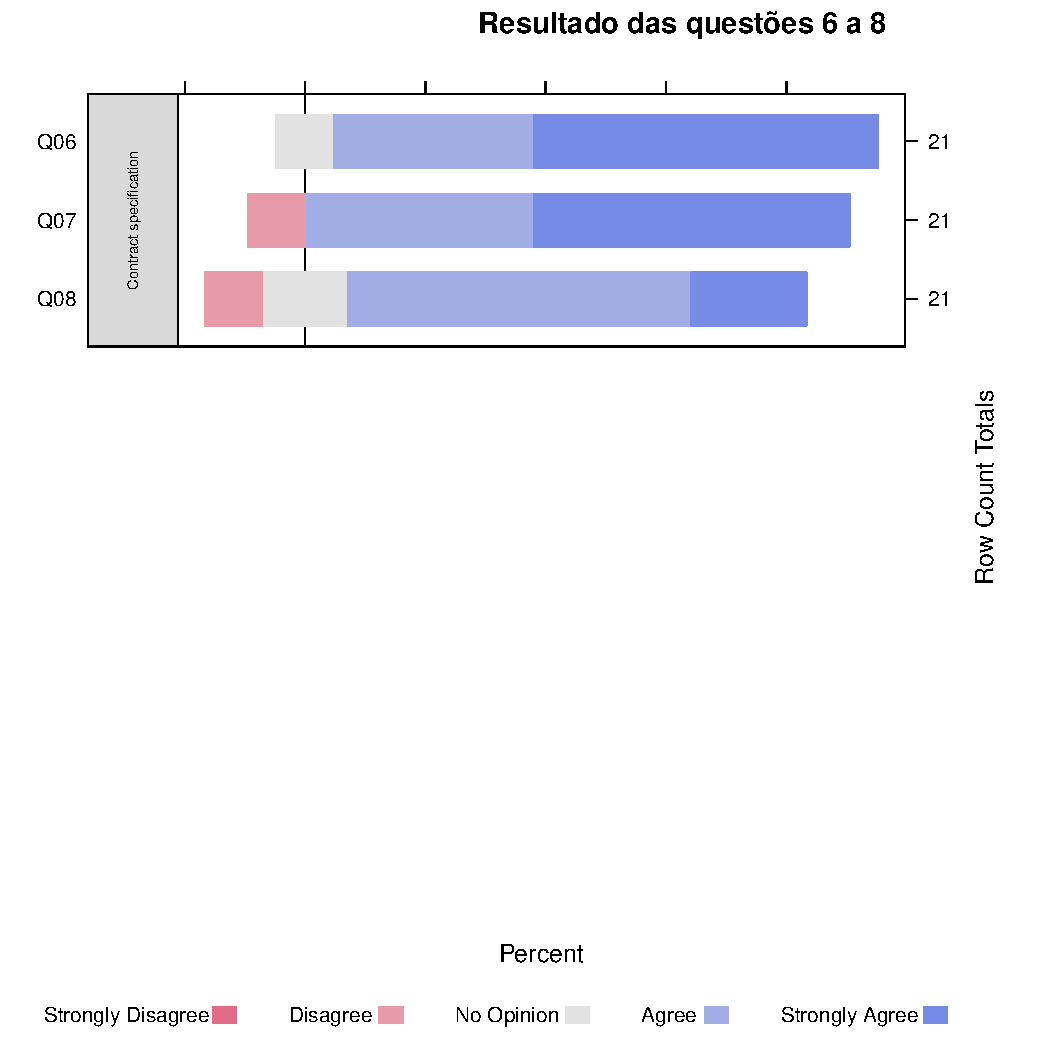
\includegraphics[width=85mm,trim = 6mm 0mm 6mm 
170mm,clip]{img/GraficoResultadoQuestoes6a8.pdf}

\caption{Gráfico com o resultado das questões 6 a 8}
\label{Respostas6a8}
\end{figure}

A questão 7 consultou a percepção dos respondentes sobre a facilidade de
identificar as operações e atributos em um contrato especificado em Swagger. A
questão 8 contém a mesma afirmação sobre um contrato especificado em \neoidl{}.
O resultado de ambas questões estão na Figura \ref{Respostas6a8} e indicam que
tanto os contratos em Swagger como em \neoidl{} são claros e fáceis de se compreender. Vale ressaltar que a maior parte dos
respondentes já possuia contato anterior com Swagger (Tabela
\ref{quantidadeRespostas5}), o que reforça o resultado positivo para a
\neoidl{}.


\subsubsection{Análise sobre aceitabilidade de construções de \designbycontract{}}

Entre as questões 9 e 12 foram feitas afirmações sobre a facilidade de se
identificar os elementos e a utilidade de se especificar pré e pós-condições em
contratos de serviços REST com a \neoidl{}. Os resultados são apresentados na
Figura \ref{Respostas9a12}. 

\begin{figure}[!htb]
\centering
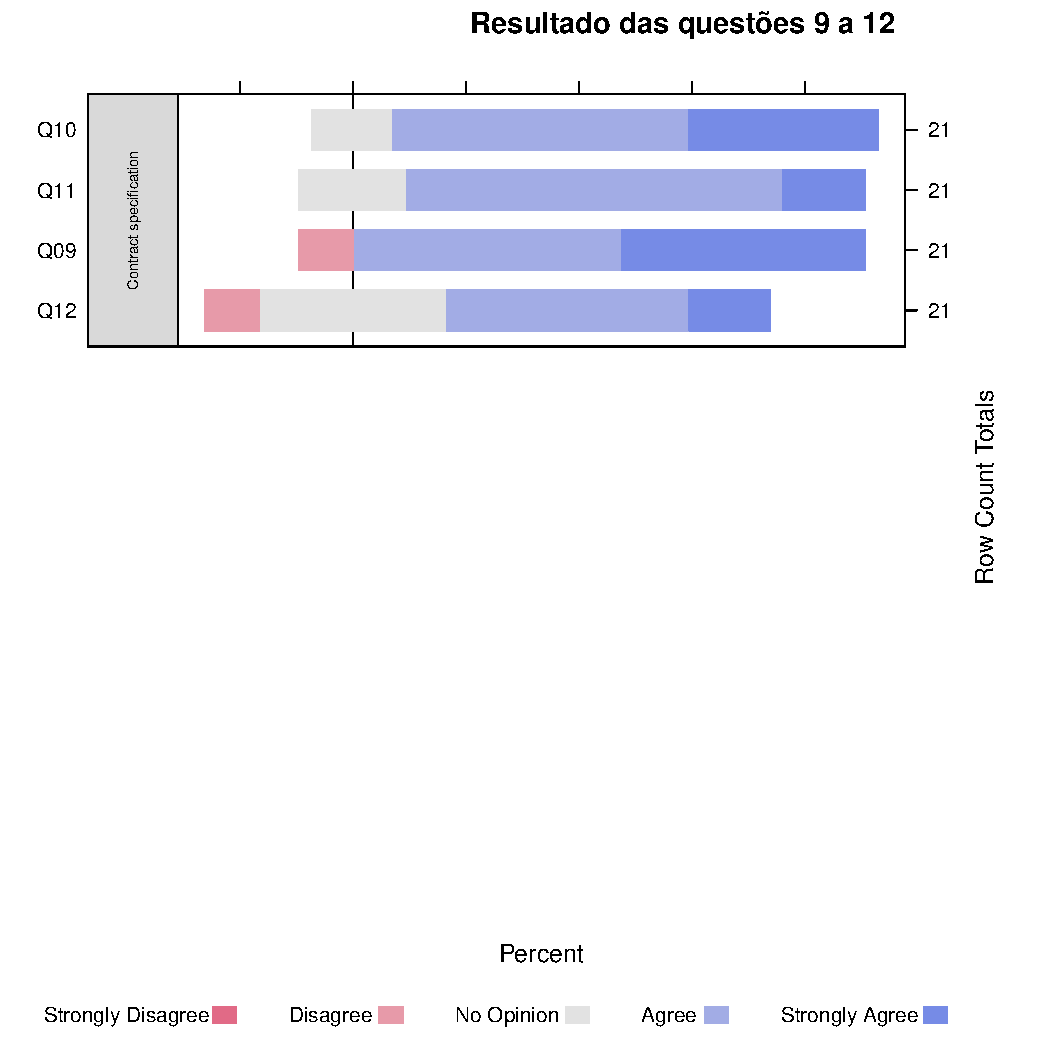
\includegraphics[width=85mm,trim = 6mm 115mm 6mm 
10mm,clip]{img/GraficoResultadoQuestoes9a12.pdf}

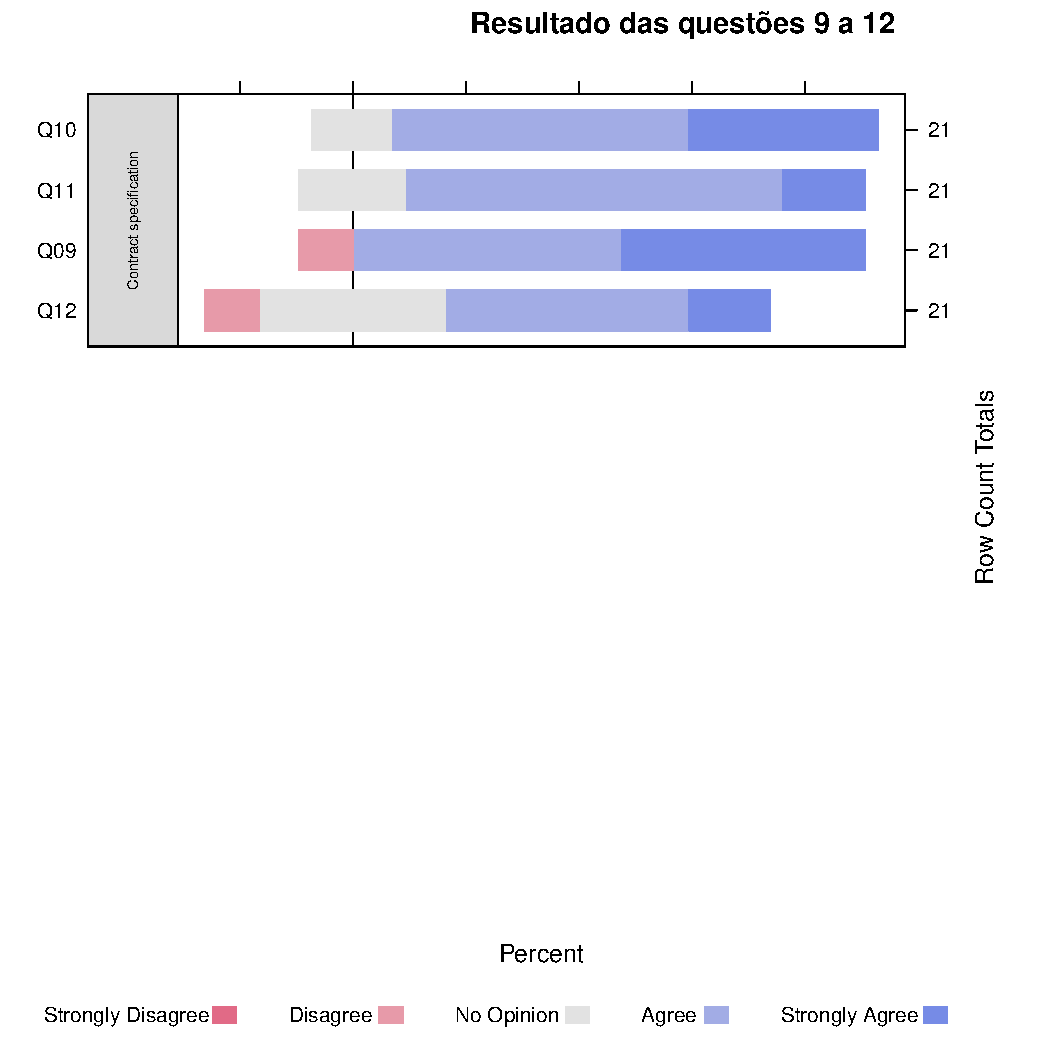
\includegraphics[width=85mm,trim = 6mm 0mm 6mm 
170mm,clip]{img/GraficoResultadoQuestoes9a12.pdf}

\caption{Gráfico com o resultado das questões 9 a 12}
\label{Respostas9a12}
\end{figure}

A questão 9 tem a afirmação de que o conhecimento explícito de precondição terá
utilidade para o desenvolvedor responsável por implementar o serviço. Quase
todos os respondentes concordaram com a afirmação, em maior e menor grau. Um
pequeno conjunto discordou, indicando que outros elementos podem ser
necessários para esse conjunto identificar a utilidade. Pode haver influência
ainda da experiência do respondente com implementação de serviços.

A afirmação da questão 10 é sobre a facilidade de se identificar pré e
pós-condições em contrato na \neoidl{}. Na questão 11, o enfoque é sobre a
facilidade de se declarar pré e pós-condições na \neoidl{}. Nos dois casos,
nenhum dos respondentes manifestou discordância, sendo que a concordância total foi mais
intensa para a afirmação da questão 10. Apenas uma pequena parcela informou que
nem concorda nem discorda da afirmação.

A questão 12 afirma que é fácil se lembrar da sintaxe de uma precondição na
\neoidl{}. Essa questão está relacionada a como se pode associar mentalmente as
construções sintáticas ao efeito que elas geram. Muito embora se esperasse um
resultado mais dividido, por ser uma construção influenciada por linguagens
diversas, os resultados indicam que a sintaxe é fácil de ser lembrada.

\subsubsection{Análise da geração de código para construções de \designbycontract{}}

Duas questões foram inseridas para tratar da utilidade da geração de código com
a \neoidl{} para contratos com suporte a \designbycontract{}. A questão 13
apontava ser claro o efeito da precondição sobre o código gerado. A maior parte
dos respondentes indicou que a geração do código para a precondição é util
em relação a produção de efeitos controláveis. A Figura \ref{Respostas13e14}
apresenta os resultados.

\begin{figure}[!htb]
\centering
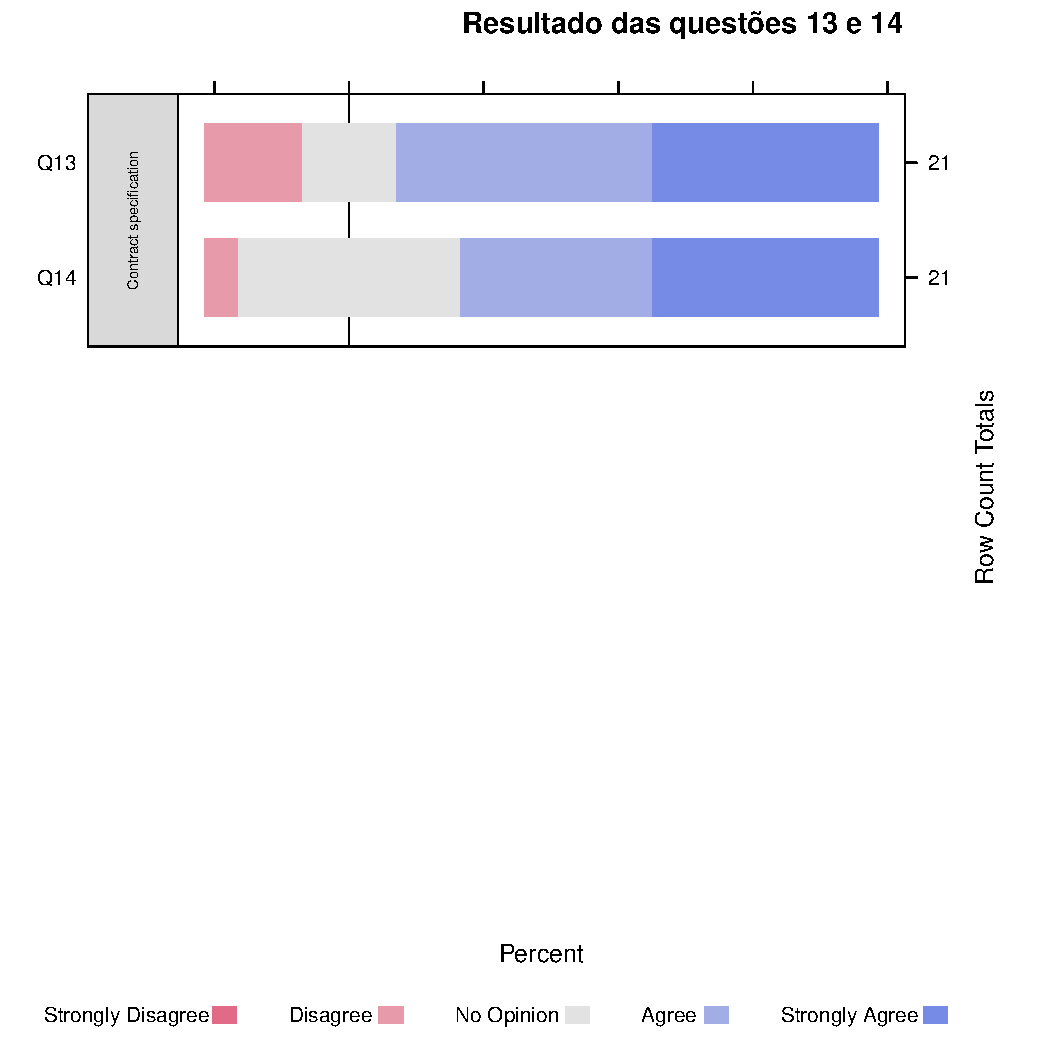
\includegraphics[width=85mm,trim = 6mm 115mm 6mm 
10mm,clip]{img/GraficoResultadoQuestoes13e14.pdf}

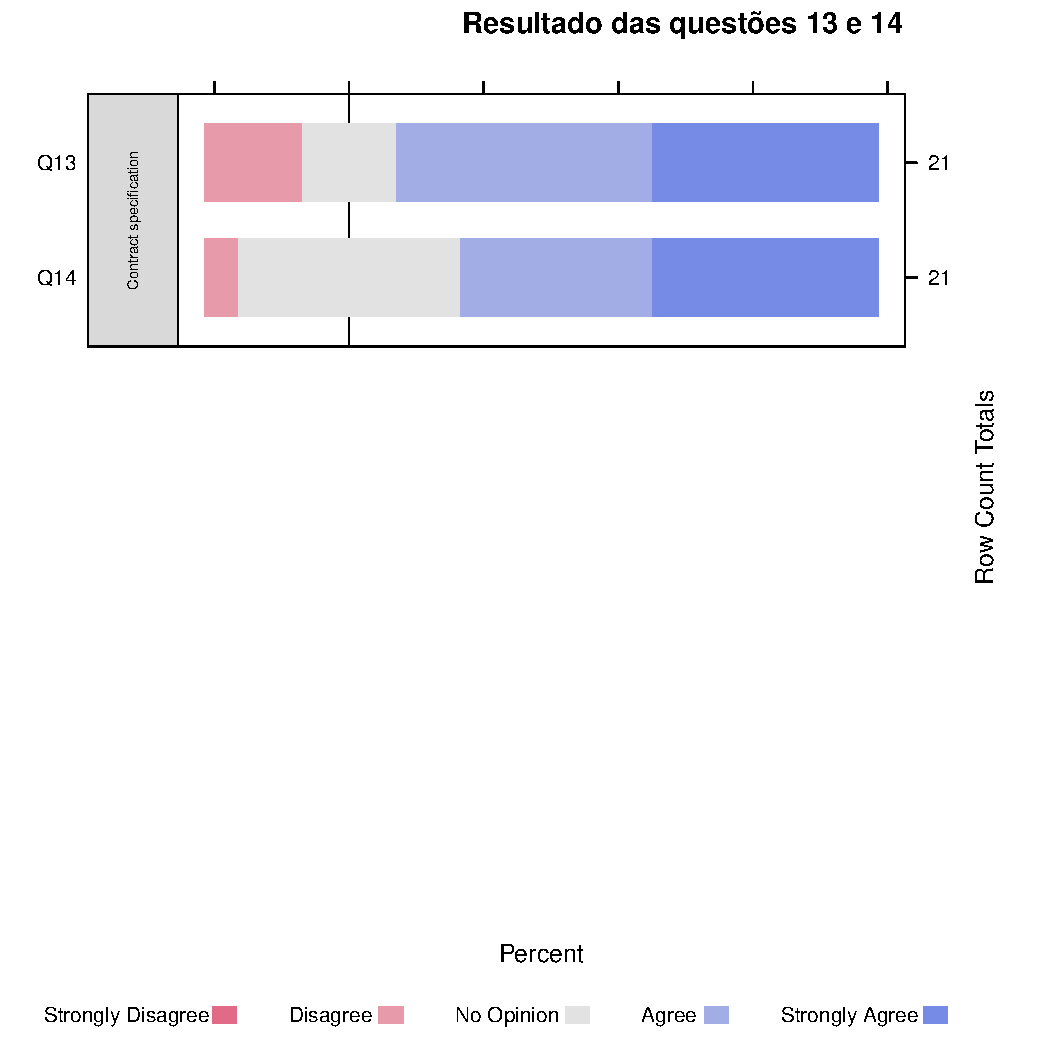
\includegraphics[width=85mm,trim = 6mm 0mm 6mm 
170mm,clip]{img/GraficoResultadoQuestoes13e14.pdf}

\caption{Gráfico com o resultado das questões 13 e 14}
\label{Respostas13e14}
\end{figure}

A questão 14 afirmou que a geração de código sobre precondições ampliará a
produtividade de implementação do serviço. O resultado apontou que uma parte
expressiva dos respondentes não concordou nem discordou. Para esses, a
especificação de precondições não incluencia a produtividade.
Por outro lado, tem-se que a maior parte concordou com a contribuição positiva
da geração de código das precondições para a produtividade. Uma parcela muito pequena discordou, ou seja,
eles acreditam que a geração de código para precondição prejudicará o
desempenho.

\subsubsection{Análise sobre a predisposição ao uso}

As duas últimas questões tratam de quão inclinado ao uso da \neoidl{} em seu
ambiente de trabalho estaria o respondente.
Esta análise é relativa \cite{laitenberger1998evaluating}, ou seja, depende de
quais os benefícios trazidos pela \neoidl{} em relação aos benefícios trazidos por soluções alternativas, como
especificação textual de contratos ou ainda por meio de Swagger. Os resultados
para essas questões são apresentadas na Figura \ref{Respostas15e16}.

\begin{figure}[!htb]
\centering
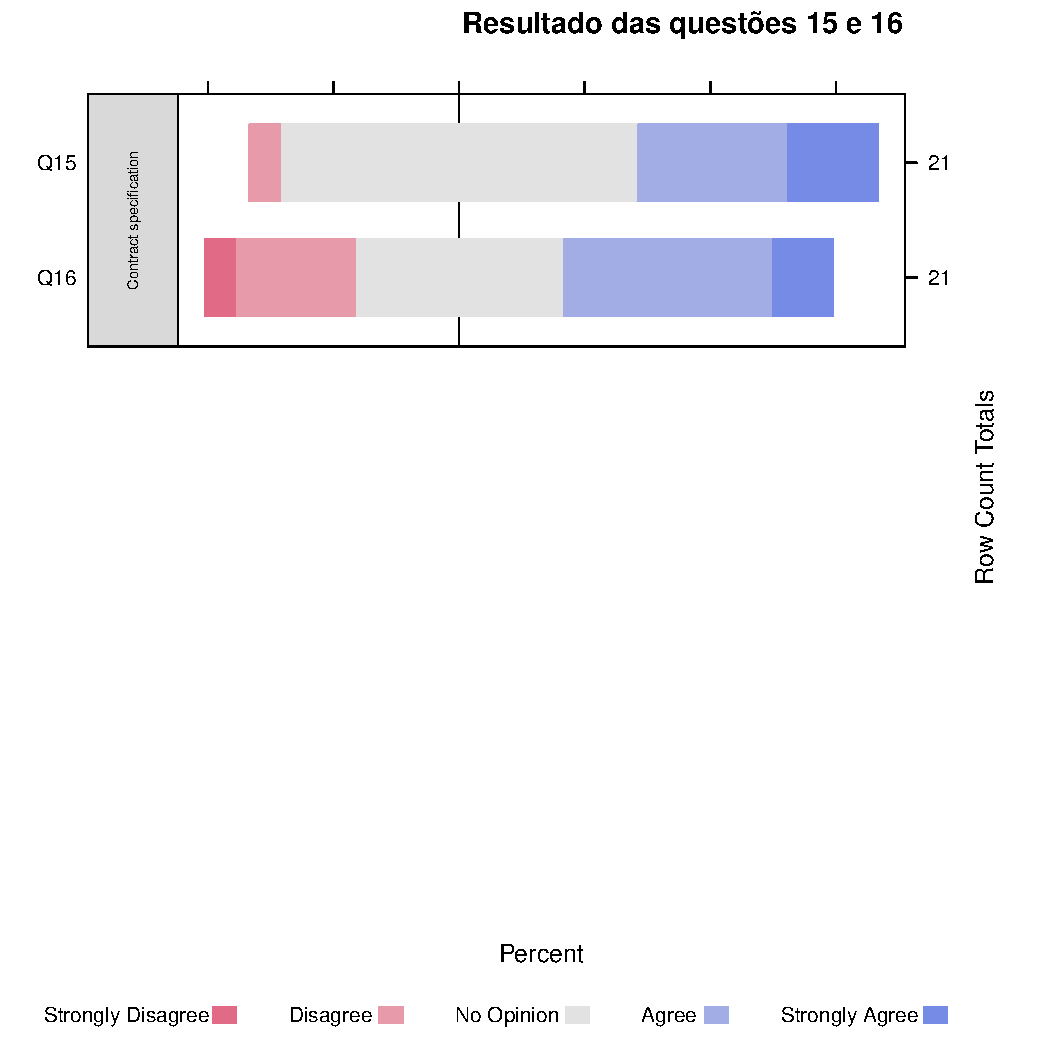
\includegraphics[width=85mm,trim = 6mm 115mm 6mm 
10mm,clip]{img/GraficoResultadoQuestoes15e16.pdf}

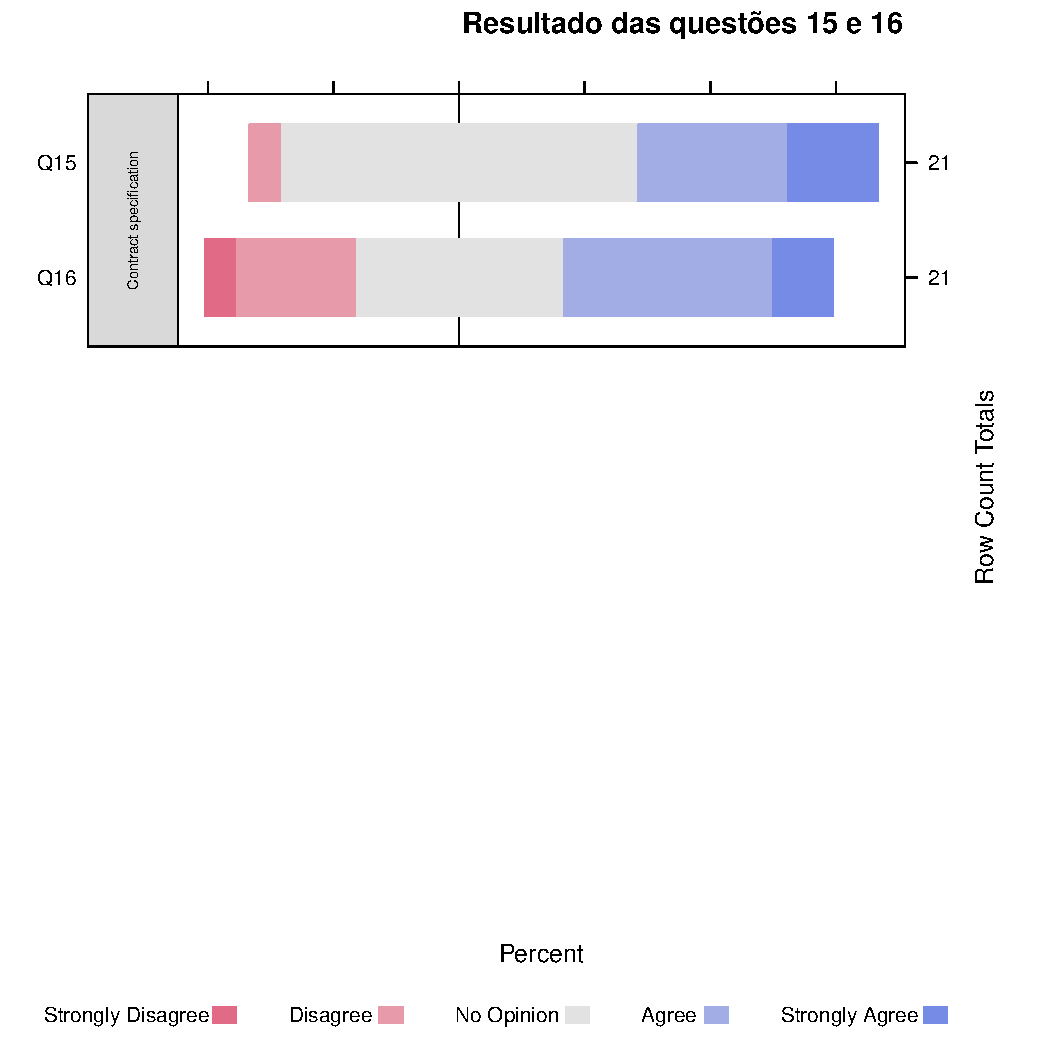
\includegraphics[width=85mm,trim = 6mm 0mm 6mm 
170mm,clip]{img/GraficoResultadoQuestoes15e16.pdf}

\caption{Gráfico com o resultado das questões 15 e 16}
\label{Respostas15e16}
\end{figure}

A questão 15 apresenta uma afirmação sobre a predisposição ao uso regular da
\neoidl{} no futuro. Pelos resultados da pesquisa, verifica-se que a maior
parcela dos respondentes nem concorda nem discorda. Esse resultado é relevante,
pois, conforme debatido anteriormente (Tabela \ref{quantidadeRespostas5}), boa
parte dos respondentes já tem contato com Swagger, que consiste em uma
alternativa direta à \neoidl{}.
Se, por um lado os respondentes não concordam prontamente em utilizar \neoidl{}, por
outro não descartam.

É necessário investigar que fatores influenciariam positivamente a predisposição
do uso da \neoidl{} e verificar se são fatores internos às empresas em que
trabalham atualmente os respondentes ou quais pontos podem ser melhorados na
\neoidl{} a fim de ampliar o nível de aceitação. Em relação às demais respostas,
nota-se uma tendência mais forte de concordância sobre o uso que regular, que
a de discordância, o que reforça o potencial de adesão ao uso da \neoidl{}.

A última questão abordou diretamente se haveria preferência de uso pela
\neoidl{} em detrimento a outras linguagens. O resultado é o mais equilibrado do
questionário, havendo uma pequena tendência para a preferência pela \neoidl{}.
O resultado da questão 16 levanta ainda outra hipótese sobre a quantidade de
respondentes em dúvida na questão 15: fatores individuais, como não lidar
diretamente com especificação de contratos, podem explicar haver um grande grupo
que não sabe informar se utilizaria regularmente a \neoidl{}.

Assim, essas questões abrem outras perspectivas de estudo, com um enfoque sobre
os fatores institucionais e o que mais poderia ser desenvolvido na \neoidl{}
para atender às necessidades das equipes de desenvolvimento.

\subsection{Ameaças}
\label{AmeacaoEstudoSubjetivo}
 
Questionários são instrumentos práticos para se realizar estudos empíricos que
visam obter a opiniões subjetivas. Uma de suas principais vantagens está em
permitir a participação de várias pessoas, ampliando a abrangência temporal e
geográfica. Há também mais domínio e facilidade de análise sobre os dados
coletados.

Entretanto, algumas ameaças podem influenciar a conclusão dos resultados. Para o
questionário aplicado neste trabalho de pesquisa, podemos destacar alguns pontos
que podem influenciar ou limitar a qualidade dos dados, bem como direcionar para
a rea\-li\-za\-ção de outros estudos empíricos sobre o tema.

Um primeiro ponto a observar é a quantidade de respondentes. Embora seja um
número superior a de alguns outros estudos avaliados
\cite{albuquerque2015quantifying}
\cite{hernandes2010avaliaccao} \cite{laitenberger1998evaluating}, uma maior
quantidade de participante ampliaria a qualidade dos dados, pois eliminaria influência de fatores muito
específicos a um conjunto de respondentes, e possibilitaria análise de 
cenários, utilizando visões de dados. O nível técnicos dos respondentes,
contudo, reduz os impactos dessa ameaça.

Outro ponto de melhoria são ações que visem proporcionar um conhecimento mínimo
sobre a \neoidl{}. Todas as respostas foram dadas apenas pelas informações
apresentadas no próprio questionário e os resultados poderiam ser diferentes se
houvesse um treinamento prévio sobre a \neoidl{}. Sob esse aspecto, tem-se que a
compreensão sobre dos elementos da sintaxe básica na \neoidl{} (questão 6) teve
resultado inferior que a compreensão dos elementos de \designbycontract{}
(questão 8). Esse resultado é inesperado, pois pressupõe-se que identificar os
elementos de \designbycontract{} só seja possível após compreender a sintaxe
básica.

Ainda, como o questionário foi aplicado apenas uma vez, não foram incluídos
pontos de melhoria a partir do primeiro conjunto de respostas para uma segunda
avaliação. Conforme debatido na Subseção \ref{AnaliseQuestionario}, algumas
questões poderiam ser inseridas em uma nova aplicação do questionário, de
modo produzir informações que permitissem conclusões mais completas.

Em estudos futuros, essas melhorias podem ser aplicadas. Em que pese esses
pontos de atenção, o estudo realizado por meio do questionário atigiu seus
resultados e produziu dados de grande relevância para o objeto em pesquisa.
